\documentclass{article}
\usepackage{icmcsmc2014}
\usepackage{times}
\usepackage{ifpdf}
\usepackage[english]{babel}
%\usepackage{cite}
\usepackage{fancyvrb}
\usepackage[autostyle]{csquotes}  
%%%%%%%%%%%%%%%%%%%%%%%% Some useful packages %%%%%%%%%%%%%%%%%%%%%%%%%%%%%%%
%%%%%%%%%%%%%%%%%%%%%%%% See related documentation %%%%%%%%%%%%%%%%%%%%%%%%%%
%\usepackage{amsmath} % popular packages from Am. Math. Soc. Please use the 
%\usepackage{amssymb} % related math environments (split, subequation, cases,
%\usepackage{amsfonts}% multline, etc.)
%\usepackage{bm}      % Bold Math package, defines the command \bf{}
%\usepackage{paralist}% extended list environments
%%subfig.sty is the modern replacement for subfigure.sty. However, subfig.sty 
%%requires and automatically loads caption.sty which overrides class handling 
%%of captions. To prevent this problem, preload caption.sty with caption=false 
%\usepackage[caption=false]{caption}
%\usepackage[font=footnotesize]{subfig}


%user defined variables
\def\papertitle{Modality Workshop}
\def\firstauthor{First author}
\def\secondauthor{Second author}
\def\thirdauthor{Third author}


% authors so far:
% Till

% adds the automatic
% Saves a lot of ouptut space in PDF... after conversion with the distiller
% Delete if you cannot get PS fonts working on your system.

% pdf-tex settings: detect automatically if run by latex or pdflatex
\newif\ifpdf
\ifx\pdfoutput\relax
\else
   \ifcase\pdfoutput
      \pdffalse
   \else
      \pdftrue
\fi

\ifpdf % compiling with pdflatex
  \usepackage[pdftex,
    pdftitle={\papertitle},
    pdfauthor={\firstauthor, \secondauthor, \thirdauthor},
    bookmarksnumbered, % use section numbers with bookmarks
    pdfstartview=XYZ % start with zoom=100% instead of full screen; 
                     % especially useful if working with a big screen :-)
   ]{hyperref}
  %\pdfcompresslevel=9

  \usepackage[pdftex]{graphicx}
  % declare the path(s) where your graphic files are and their extensions so 
  %you won't have to specify these with every instance of \includegraphics
  \graphicspath{{./figures/}}
  \DeclareGraphicsExtensions{.pdf,.jpeg,.png}

  \usepackage[figure,table]{hypcap}
\fi

%setup the hyperref package - make the links black without a surrounding frame
\hypersetup{
    colorlinks,%
    citecolor=black,%
    filecolor=black,%
    linkcolor=black,%
    urlcolor=black
}


% Title.
% ------
\title{\papertitle}

% Authors
% Please note that submissions are NOT anonymous, therefore 
% authors' names have to be VISIBLE in your manuscript. 
%
% Single address
% To use with only one author or several with the same address
% ---------------
%\oneauthor
%   {\firstauthor} {Affiliation1 \\ %
%     {\tt \href{mailto:author1@smcnetwork.org}{author1@smcnetwork.org}}}

%Two addresses
%--------------
% \twoauthors
%   {\firstauthor} {Affiliation1 \\ %
%     {\tt \href{mailto:author1@smcnetwork.org}{author1@smcnetwork.org}}}
%   {\secondauthor} {Affiliation2 \\ %
%     {\tt \href{mailto:author2@smcnetwork.org}{author2@smcnetwork.org}}}

% Three addresses
% --------------
 \threeauthors
   {\firstauthor} {Affiliation1 \\ %
     {\tt \href{mailto:author1@smcnetwork.org}{author1@smcnetwork.org}}}
   {\secondauthor} {Affiliation2 \\ %
     {\tt \href{mailto:author2@smcnetwork.org}{author2@smcnetwork.org}}}
   {\thirdauthor} { Affiliation3 \\ %
     {\tt \href{mailto:author3@smcnetwork.org}{author3@smcnetwork.org}}}

\newcommand{\todo}[1] {\emph{\textbf{TODO:} #1}}
\DefineShortVerb{\|}


\begin{document}
%
\capstartfalse
\maketitle
\capstarttrue
%
\begin{abstract}
The Modality Toolkit aims to improve and facilitate the use of digital technology within interactive sound art and music. 
Written in SuperCollider, it simplifies the creation of individual electronic instruments by combining custom sound engines with off-the-shelf controllers. 
To this end, a common code interface, |MKtl|, is used to connect controllers from various sources and protocols. 
Currently, HID and MIDI are supported; GUI-based interfaces can be created on the fly from interface descriptions.

In the workshop, the toolkit is introduced and used by participants to lay out their control ideas and play music with each other.
\end{abstract}

\begin{figure}[h]
	\centering
		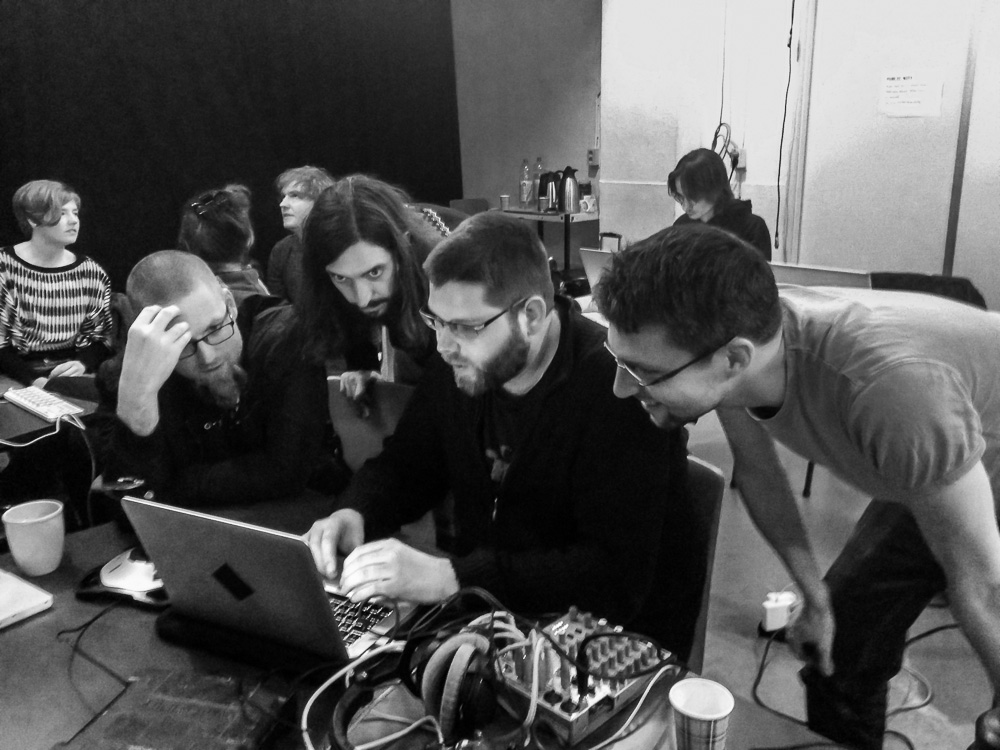
\includegraphics[width=\columnwidth]{../media/20140403-IMG_1667.jpg}
	\caption{Public workshop and open Lab at STEIM}
	\label{fig:media_20140331-IMG_5976}
\end{figure}






\section{Overview of the modality concept and its aims}
\label{sec:overview_of_modality_concept_and_aims}

Modality is a project dedicated to modal interaction with synthesis processes for physical control in performance. 
Its primary product is the Modality Toolkit, a library to facilitate straightforward access to hardware controllers in the SuperCollider programming language. 
It is designed and developed by the ModalityTeam, a group of people that see themselves as both users and developers both of and for SuperCollider.

The idea behind the Modality Toolkit is to simplify the creation of individual electronic instruments using controllers of various kinds. 
To this end, a common code interface, MKtl, is used for connecting controllers from various sources and protocols. 
Currently HID and MIDI are supported with OSC, GUI-based interfaces can be created on the fly from interface descriptions.


\section{Scope of Modality}
\label{sec:scope_of_modality_tech_info_where_what}



\section{Workshop content}
\label{sec:workshop_content}

The concept of the workshop is to be as “hands-­on” as possible.
Participants will learn how to use the Modality toolkit, create their own instruments, and play together with their creations. 
Under the guidance of the Modality Work Group, each participant will be able to work on his or her own instrument, and use and play it along with the other participants.

In detail, the outline of the workshop is as follows:

\begin{itemize}
	\item brief introduction to the Modality toolkit,
	\item installation party,
	\item mapping out devices (i.e., writing description files for them), in case the brought devices are not yet specified in Modality (contributing to the library of known devices),
	\item accessing devices and using data from devices; creating a basic sound--controller setup,
	\item performing with the system,
	\item swap controllers and share sounds between participants,
	\item adaption of the setup and manipulation of data streams,
	\item performing with the system
\end{itemize}



Participants should bring 
\begin{itemize}
	\item MIDI or HID controllers such as game gads, joysticks or fader boxes, 
	\item their own laptops with a recent version of SuperCollider installed, and
	\item a basic familiarity with the programming environment SuperCollider.
\end{itemize}


\begin{acknowledgments}
The Modality team is (in alphabetical order):
    Marije Baalman,
	Tim Blechmann,
    Till Bovermann,
    Alberto de Campo,
    Jeff Carey,
    Bjoernar Habbestad,
	Dominik Hildebrand Marques Lopes,
	Amelie Hinrichsen,
    Robert van Heumen,
    Hannes Hoelzl,
    Miguel Negrao, and
    Wouter Snoei.
Associated organisations are (in alphabetical order):
BEK,
the project \emph{Design, Development and Dissemination of New Musical Instruments} of UdK Berlin/TU Berlin, supported by the Einstein Foundation,
nescivi supported by theCreative Industry Fund NL, and
STEIM.

\end{acknowledgments} 

%%%%%%%%%%%%%%%%%%%%%%%%%%%%%%%%%%%%%%%%%%%%%%%%%%%%%%%%%%%%%%%%%%%%%%%%%%%%%
%bibliography here
\bibliography{smacsmc2014template}

\end{document}
